
	\documentclass[a4paper,titlepage]{article}
%packages
	\usepackage{amsmath, amssymb, amsfonts}
	\usepackage[ngerman]{babel}
	\usepackage[usenames]{color}
	\usepackage[utf8]{inputenc}
	\usepackage{listings}
	\usepackage{graphicx}
	%Kopf und Fusszeile
	\usepackage{fancyhdr}
	%Seitenabstaende (margins)
	\usepackage[left=3cm,right=2cm,top=2cm,bottom=2cm,includeheadfoot]{geometry}

%pagestyle fuer Kopf und Fusszeile
	\pagestyle{fancy}
	\fancyhf{}
	%Kopfzeile
		\fancyhead[L]{OpenGL EERT}
		\fancyhead[R]{Robert Schadek}
		\renewcommand{\headrulewidth}{0.5pt}
	%Fusszeile
		\fancyfoot[C]{Seite \thepage}
		\renewcommand{\footrulewidth}{0.5pt}
%Titel
\title{
	{\huge OpenGL EERT\\
	\huge - Einzelprojekt -\\
	{\large Universit\"at Oldenburg}\\
	\large Wintersemester 2008/2009\\
	%Abgabe: 18.01.2008\\
	}
	\date{\today}
	\author{\\
		\large 	Robert Schadek\\
	}
}

%Sonstiges
	% keine Einrckung bei neuen Abstzen
	\setlength{\parindent}{0em}



%Dukumentanfang
\begin{document}
%Titel erzeugen und danach eine neue Seite bgeinnen
\maketitle
\tableofcontents
\section{Einleitung, Projektziel}
Der Name meines Projektes lautet EERT. Dies steht f"ur EERT enhanced rendering technology.
Die Idee hinter dem Projekt ist jene, dass ich ein Programm schaffen wollte, welches in der Lage ist
neue Szenen darstellen zu k"onnen, ohne jedes mal neu kompiliert zu werden. Au"serdem wollte ich Frustum 
Culling implementieren, da dies, wie ich finde, zu jeder Grafikanwendung geh"ort die Echtzeit f"ahig 
sein will. Au"serdem wollte ich in der Lage sein eine Szene darzustellen die theoretisch aus mehr als einer
Millionen Triangle besteht und dies mit Frameraten "uber 100FPS.\\

\section{Techniken}
\subsection{Allgemein}
Zu den verwendeten Techniken kann man allgemein sagen, dass ich nicht versucht habe, auf biegen und brechen, 
jede vorgestellte Technik aus der Vorlesung in mein Projekt einzubauen. Ich habe vielmehr versucht Techniken 
zu implementieren, die nicht vorgestellt wurden, allerdings angesprochen.

\subsection{Szenenbeschreibung}
Meine Szenenbeschreibung sieht so aus, dass ich mir eine Dateistruktur ausgedacht hab in der man speichern 
kann welches Objekt geladen wird, welche Texturen zu ihm geh"oren, wo sich die Objektinstanzen befinden, wie 
sich jene verschieben und rotieren usw. Um mir die Arbeit einfacher zu machen habe ich mich mir das .obj Format 
als Vorbild genommen. Die Szenendatein tragen die Endung .eob was f"ur eert objekt seht.\\
Intern sind diese wie folgt aufgebaut:\\

\textbf{l float float float float float float}\\
Erzeugt ein direktionales Licht, wobei die ersten drei floats die Richtung und die zweiten drei die Farbe angeben.\\

\textbf{p long float float float float float float float float}\\
Erzeugt einen Pfad auf dem sich die Kamera bewegt. Der long Wert gibt an wie lange es in Millisekunden dauert
bis sich die Kamera vom ersten bis zum dritten Vektor bewegt hat. Es m"ussen mindestens drei Vektoren oder anderes
gesagt neun floats angegeben werden. Es k"onnen dann zus"atzlich jeweils drei weitere Vektoren angegeben werden.\\

\textbf{a float float float float float float float float float}\\
Erzeugt einen Pfad auf den die Kamera guckt, w"ahrend sie sich "uber den unter p deklarierten Pfad bewegt.
Es sind hier genau so viel Vektoren zu deklarieren wie f"ur den Pfad. Die Bewegungsgeschwindigkeit ist jene
unter p deklarierte.\\

\textbf{o *.obj *.obj *.obj *.obj *.obj *.obj}\\
Dies erzeugt ein Objekt die sechs *.obj geben jeweils die Dateinamen der Objekte an. Wobei diese Aufgrund des
Verwendeten LOD Verfahrens(siehe Unten) vom hochaufl"osend absteigent sortiert sind.\\

\textbf{ot *.png *.png *.png *.png *.png *.png}\\
Hiermit werden die Texturen für das als n"achste Deklarierte Objekt gesetzt. Wie bei den Objekten sollten sechs
Aufl"osungen für die verschiedenen LOD Aufl"osungen vorgehalten werden.\\

\textbf{oi int float float float float float float float float float float float float}\\
Eine mit oi beginnende Zeile beschreibt eine Objektinstanz. Das int zu beginn gibt Auskunft "uber, dass
dazugeh"ohrige Objekt. Die n"achsten drei floats beschreiben den Startvektor gefolgt von der Startrotation
und der Konstanten Rotation. Alle folgenden drei floats beschreiben eine Bewegungsrichtung.\\

\subsection{Editor} 
Der Editor entstand, als es klar wurde, dass ich eine Vielzahl von Objektinstanzen in meiner Beispielszene darstellen
wollte. H"atte ich diese per Hand geschrieben, h"atte ich f"ur jede Objektinstanz mindestens neun floats eingeben m"ussen. 
Um dies ein wenig zu vereinfachen, habe ich einen kleinen Editor geschrieben der dies "ubernimmt.
Die Hauptaufgabe des Editors ist es Positionen innerhalb der Szene zu finden in denen nicht bereits ein Objekt
plaziert ist. Aufgrund von Webstart ist es nicht m"oglich den Editor zu demonstrieren. Dies ist deshalb der Fall, 
da Webstart nicht den Zugriff auf das lokale Datensystem erlaubt und die durch den Editor erstelle Datei noch ein wenig
manuellen Eingriff ben"otigt, bis sie darstellbar ist.


\subsection{Objektloader}
Der Implementierte Objektloader ist in der Lage jede Form von Mesh zu laden, solange sie nur aus Dreiecken 
besteht und geschlossen sind. Die Geschlossenheite ist Voraussetzung f"ur Shadow Volumen.
Wie oben bereits angedeutet lade ich Objekte des Typs \textbf{.obj}. Ich habe dieses Format gew"ahlt, da es 
recht einfach zu verstehen ist und f"ur meine Zwecke vollkommen ausreicht. 

\subsection{Szenenmusik}
Damit die Szene nicht zu steril wirkt, habe ich mit Hilfe der Jlayer Libray die Wiedergabe von MP3 Datein
implementiert. Da dies kein Feature von OpenGL ist, werde ich hier nicht weiter drauf eingehen. 

\subsection{Per Pixel Lightning}
Wie die "Uberschrift es bereits andeutet, ist die Beleutung durch Per-Pixel Lightning realisieren. 
Aus dem einfachen Grund, da dies zur Zeit Stand der Technik ist. Da die Demoszene ein Skybox
enth"allt die einen Himmel darstellt, hab ich das Per Pixel Lightning f"ur direktionales Licht implementiert.

\subsection{Objektinstanzen}
Unter Objektinstanzen hat man eine Technik zu verstehen, die es mir erm"oglicht einen Mesh nur einmal im 
Speicher zu halten, ihn aber an vielen Stellen der Szene mit verschiedenen Eigenschaften zu zeichnen. Dies 
ist Sinnvoll,da die Objekte die ich in einer Szene laden alleine ca. 2MB gro"s sind. Nimmt man nun an man w"urde 
dieses Objekt 400 mal laden um es an 400 Stellen zu zeichnen br"aucht ich alleine ca. 800MB Speicher nur 
f"ur die Objektdaten. 400 mal deshalb da ich in der Demoszene 400 Objektinstanzen darstelle.\\
Dank der Objektinstanzen muss ich die Objektdaten nur einmal laden. F"ur jede Instanz muss prinzipiell nur noch 
ein Postions- sowie Rotationsvektor gespeichert werden.

\subsection{UV-Texturing}
Beim UV-Texturing oder wie es auch genannt wird UV-Mapping, wird ein komplexes 3D Objekt derart auseinander 
gefallt, dass er sich auf einer 2D Fl"ache sprich Textur darstellen l"asst. Dies erm"oglicht es Objekte zu 
texturieren ohne dabei auf den Hilfsmittel von OpenGL zur"uckzugreifen. Dies macht Sinn, da es mit diesen 
Hilfsmitteln nicht m"oglich ist, die Texturen beliebig komplex auf Objekten abzubilden. Das UV-Mapping steht 
in enger Verbindung mit dem Objektloader, da beim Erstellen der Objekte bereits die sogenannte UV-Map erstellt 
werden muss. Dies kann dann sp"ater in einem beliebigen Zeichnenprogramm bearbeitet werden.\\

Hier ein Beispiel f"ur eine solche UV-Texture.\\

\includegraphics[width = 1.0\textwidth]{t10138u_Suzanne.png}\\

\subsection{Level of Detail}
Level of Detail kann man als Mipmapping f"ur Dreiecke verstehen. Ich setze voraus, dass jedes Objekt welches 
in EERT darstellt werden soll, in sechs Aufl"osungen vorliegt. Beispielhaft von 10000 bis 300 Dreiecken. Dies 
mache ich mir so zu nutze, indem ich sage, wenn ein Objekt so weit von der Kamera entfernt ist, dass es nur noch 
wenige Pixel auf dem Bildschirm einnimmt, braucht es nicht aus mehrere tausend Dreiecken bestehen, es reicht 
wenn jenes aus ein paar hundert besteht.
Betrachtet man nun mehrere diese Stufen f"allt es dem Benutzer nicht auf, dass bei bestimmen Abst"anden von 
der Kamera eigentlich verschiedene Objekte gezeichnet werden. Mit Abstand ist die Euklidische Distanz zwischen
Kamerapostion und Objektmittelpunkt gemeint.

\subsection{Shadow Volumes}
Shadow Volumes ist eine Technik zum darstellen von Schatten. Die Technik funktioniert so, dass ausgehend von 
einer Lichtquelle die Silhouette eines jeden Objekt extrudiert wird und der dadurch entstandene Körper als nicht
durch die entsprechende Lichtquelle beleuchtet wird. Eine genauere Beschreibung w"urde den Umfang dieses Dokuments
platzen lassen. Dieses Feature ist aufgrund eines Fehler nicht in der Engine aktiviert.

\subsection{Octree}
Die Idee hinter dem Octree ist es, den Raum in dem sich die zu zeichnen Objekte befinden in acht Unterr"aume 
aufzuteilen. Nachdem der Raum das erste mal aufgeteilt wurde wird "uberpr"uft welche Objekte in welche Unterraum 
liegen. Danach wird jeder Unterraum wiederum in acht Unter"aume aufgeteilt und es wird erneut "uberpr"uft 
welche Objekte sich in ihm befinden. Dies wird solange fortgef"uhrt bis eine bestimmte Rekursionstiefe 
erreicht ist oder ein Unterraum leer ist. Es ist darauf zu achten was f"ur eine Rekursionstiefe man w"ahlt 
da die Anzahl der Knoten mit 
$O(8^n)$ w"achst.\\

In dieses Bild wird die Raumeinteilung aus dem Inneren des Octrees dargestellt.\\
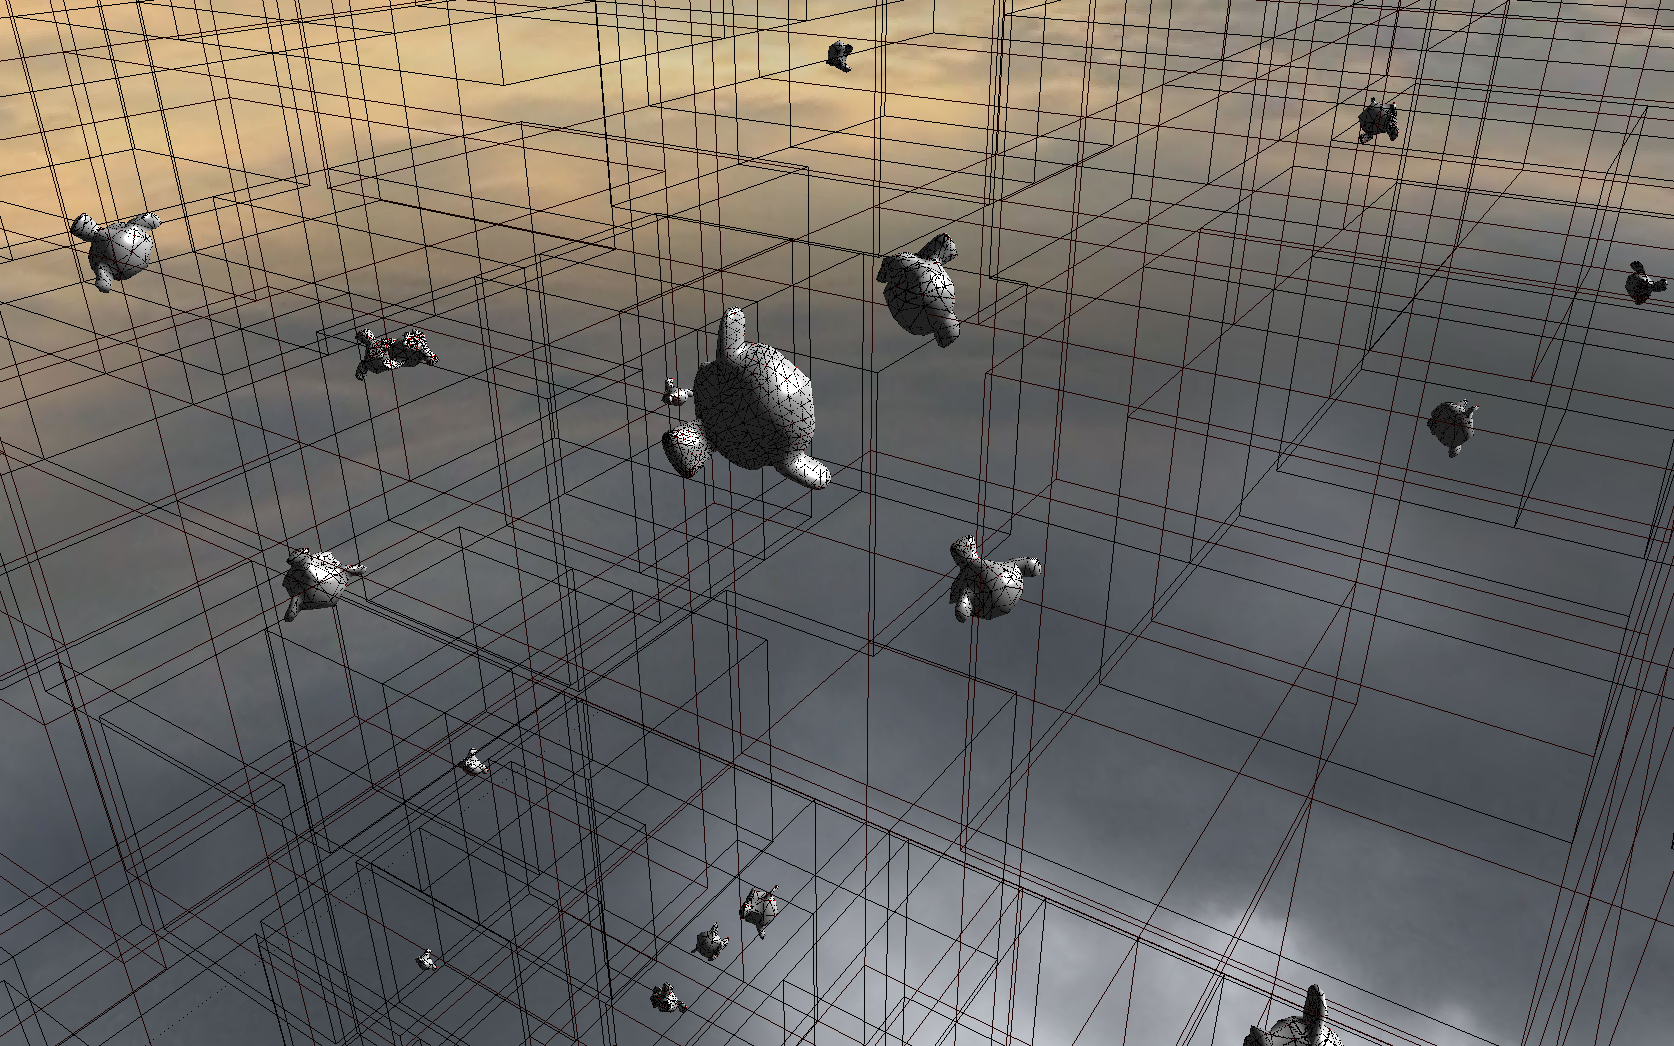
\includegraphics[width = 1.0\textwidth]{oc1.png}\\

Beim Rendern "uberpr"uft man nun, ob sich die Root-node im Frustum der Kamera befindet, ist dies nicht so ist 
der Rendervorgang bereits vorbei, da es ausgeschlossen ist, dass sich irgendeine weitere Node und somit 
irgendein Objekt im Frustum befindet. Sollte sich eine Node im Frustum befinden werde alle ihre Kinder 
"uberpr"uft. Dies geschieht solange bis die "Uberpr"uft Node keine Kinder mehr hat, sollte sie dies jeweilige Node
immer noch im Frustum befinden werden alle Objekte die sich in ihr befinden gezeichnet.\\

Dies erm"oglicht ein "uberaus effektives Frustum Culling. Die Datenstruktur ist zudem so schnell aufzubauen, 
dass es m"oglich ist, diese jedem Frame neu aufzubauen. Somit k"onnen alle Objekte frei bewegt werden.\\

Die Datenstruktur eignet sich nicht nur f"ur das Frustum Culling zus"atzlich ist es auch eine effiziente Technik
f"ur das "Uberpr"ufen von Kollisionen.

Dieses Bild zeigt den Octree von au"sen. Wie man sieht es er kein vollst"andiger W"urfel was sich durch die 
Leerheit einzelner Nodes erkl"aren l"asst.\\
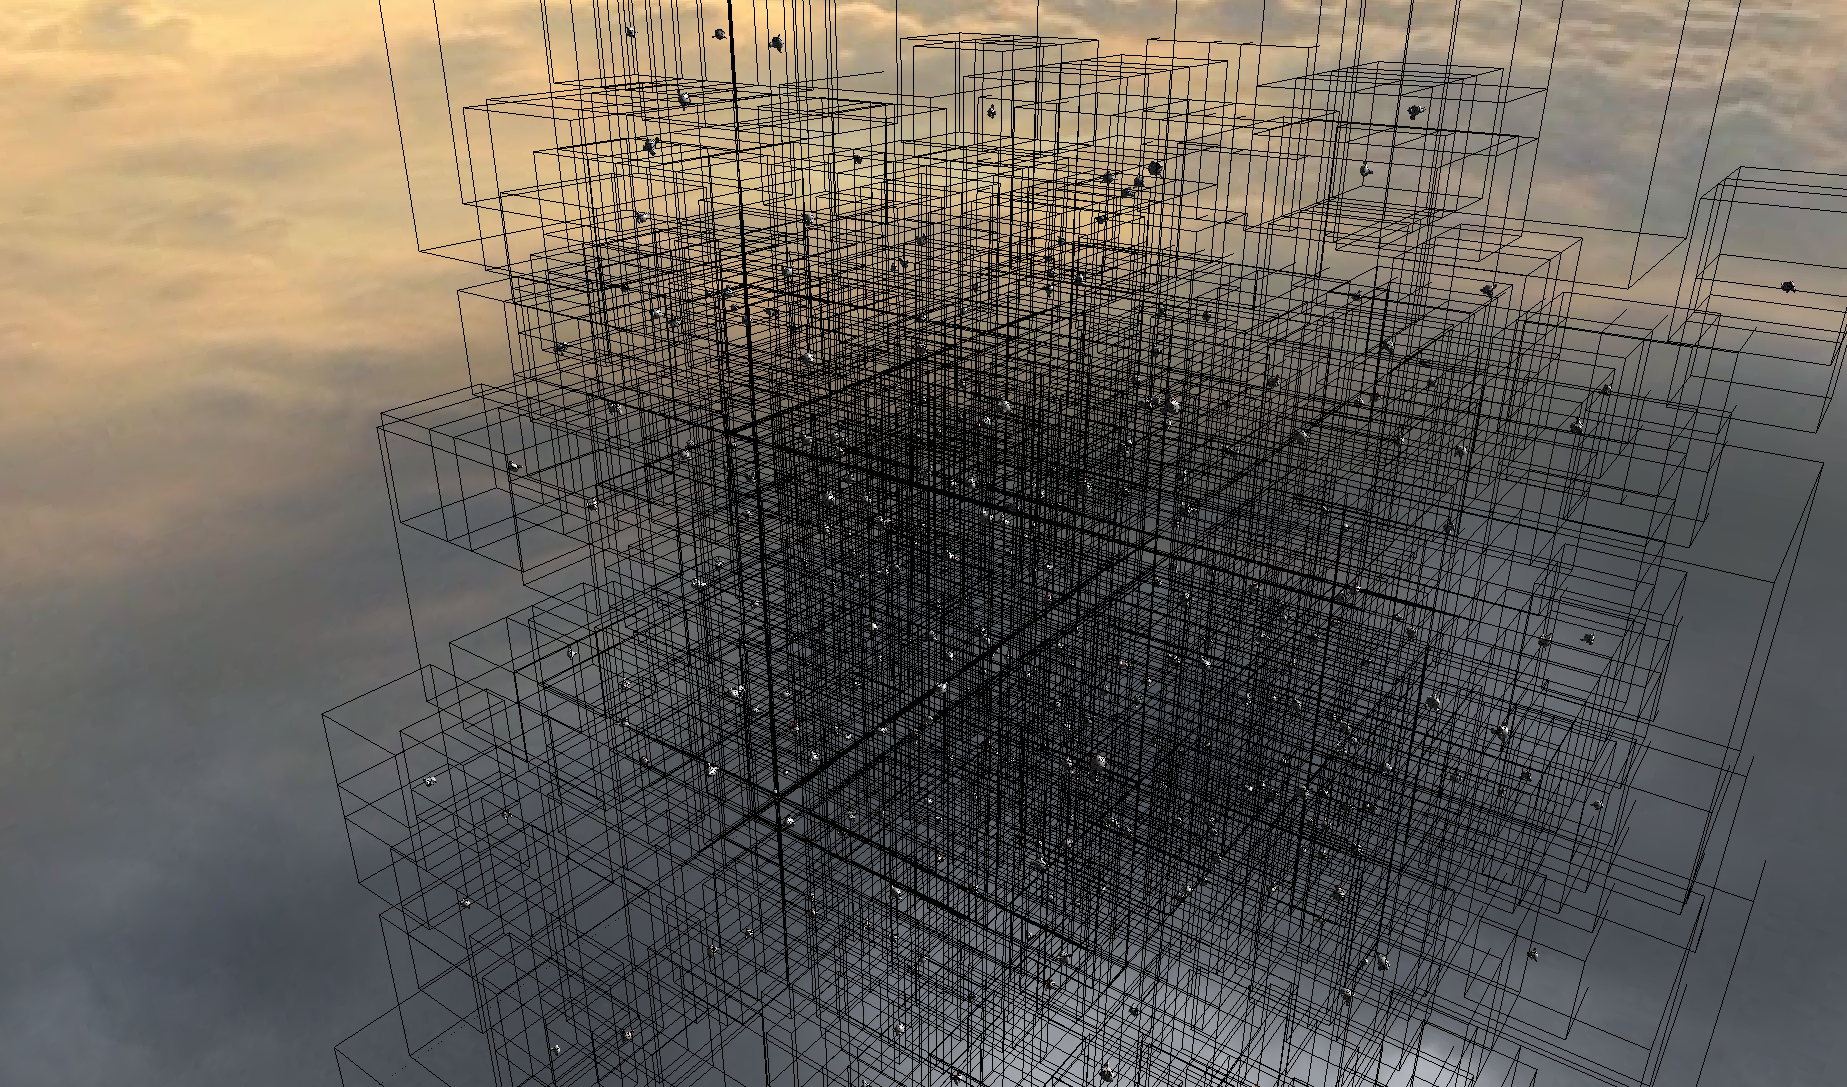
\includegraphics[width = 1.0\textwidth]{oc2.png}

\section{Schluss}
Die Bedienung des Programmes wird im Programm erkl"art. Der Programmcode sowie die Modele und Texturen sind 
unter git://github.com/burner/eert.git zu erhalten. 
\end{document}
